\documentclass[9pt]{beamer}
\usetheme{Berlin}
\usepackage{multicol}
\usepackage{graphicx}
\linespread{1.35}
\usepackage{amsmath}
\usepackage{color}
\usepackage{xcolor}
\usepackage{tikz}
\usetikzlibrary{arrows,automata}


\begin{document}
\begin{frame}

\begin{flushright}
 \texttt{Finite State Machine} \hspace*{0.10cm}\textbf{$|$} \textbf{77}\hspace*{0.5cm}
\end{flushright}

\section*{Transitional Format}

\vspace*{1cm}
\begin{center}
\section{picture}
\includegraphics[width=8cm,height=2.5cm]{77-1.png}
\end{center}

\vspace*{0.5cm}
\textbf{Step III:} Repeat these steps for each of the states. By this process, the Mealy machine-equivalent Moore
machine is constructed. The process is described in Fig.3.31.\\
\hspace*{0.2cm} Consider the following examples.
\end{frame}

\begin{frame}
\fcolorbox{red}{blue}{\textbf{Example 3.21}}\hspace*{0.1cm} \texttt{\small{Convert the following Moore machine into an equivalent Mealy machine as given in Fig. 3.32.}}
\begin{center}
\section{picture}
\includegraphics[width=5cm,height=3cm]{77-2.png}
\end{center}

\pause
\textbf{Solution:}

\small{\fcolorbox{white}{blue}{\textcolor[rgb]{1.00,1.00,1.00}{1}.}In this machine, A is the beginning state. So, start from
A. For A, there are two incoming arcs, from C to A
with input b and another in the form of the start-state
indication with no input. State A is labelled with output
$0$. As the start-state indication contains no input, it is
useless and, therefore, keep it as it is.\\
\hspace*{0.2cm} Modify the label of the incoming edge from C to
B including the output of state A. So, the label of the
incoming state is C to A with label $b/0$.}

\end{frame}

\begin{frame}
\fcolorbox{white}{blue}{\textcolor[rgb]{1.00,1.00,1.00}{2}.} State B is labelled with output $1$. The incoming edges
to the state B are from A to B with input a, B to B with
inputs a and b, and C to B with input a.\\
\hspace*{0.2cm} Modify the labels of the incoming edges including
the output of state B. So, the labels of the incoming
states become A to B with label $a/1$, B to B with labels
$a/1$ and $b/1$, and C to B with label $a/1$.\\
\fcolorbox{white}{blue}{\textcolor[rgb]{1.00,1.00,1.00}{3}.} State C is labelled with output $0$. There is only one
incoming edge to this state, from A to C with input b.
The modified label is $b/0$.\\
\hspace*{0.2cm} The converted Mealy machine is given in Fig. 3.33.

\pause
\begin{center}
\section{picture}
\includegraphics[width=5cm,height=3cm]{77-3.png}
\end{center}
\end{frame}

\begin{frame}
\fcolorbox{red}{blue}{\textbf{Example 3.22}}\hspace*{0.1cm} \texttt{ Convert the following Moore machine into an equivalent Mealy machine as given in
Fig. 3.34.}
\pause
\begin{center}
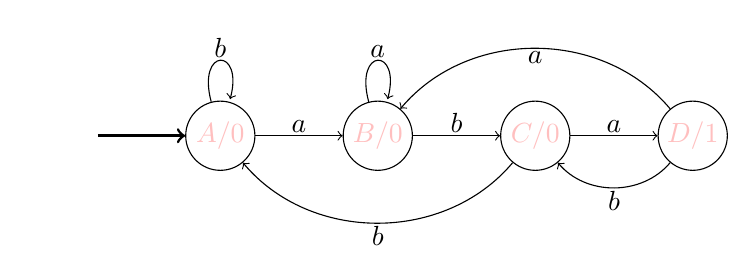
\begin{tikzpicture}[node distance = 2cm,auto,inner sep=1pt]
\node[state,draw=white,inner sep=0pt] (A) {$$};
\node[state,text=pink,draw=black] (B) [ right of = A]  {$A/0$};
\node[state,text=pink,draw=black] (C) [right of = B]  {$B/0$};
\node[state,text=pink,draw=black] (D) [right of = C]  {$C/0$};
\node[state,text=pink,draw=black] (E) [right of = D]  {$D/1$};

\path (A) edge [->,line width=1pt,node distance = 0.1cm] node {$$} (B);
\path (B) edge [->,loop above] node {$b$} (B);
\path (B) edge [->] node {$a$} (C);
\path (C) edge [->,loop above] node {$a$} (C);
\path (C) edge [->] node {$b$} (D);
\path (D) edge [->] node {$a$} (E);
\path (E) edge [->,bend left=50] node {$b$} (D);
\path (D) edge [->,bend left=50] node {$b$} (B);
\path (E) edge [->,bend right=50] node {$a$} (C);
\end{tikzpicture}
\end{center}
\begin{center}
\textbf{Fig. 3.34}
\end{center}
\end{frame}

\begin{frame}
\section*{Transitional Format}
\begin{flushleft}
    \textbf{78}\hspace*{0.1cm} \textbf{$|$} \hspace*{0.1cm} \texttt{Introduction to Automata Theory, Formal Languages and Computation}
  \end{flushleft}

\vspace*{0.5cm}
\textbf{Solution:} State A is labelled with output $0$. The incoming edges to this state are C to A for input b, A to
A for input b, and one as start-state indication with no input. Ignore the edge with start-state indication.\\
 \hspace*{0.2cm} Modify the labels of the incoming edges by including the output of state A. So, the modified labels
become A to A with label $b/0$ and C to A with label $b/0$.\\
 \hspace*{0.2cm} State B is labelled with output $0$. The incoming edges to this state are A to B for input a, B to B for
input a, and D to B for input a. The modified labels are A to B with label $a/0$, B to B with label $a/0$, and
D to B with label $a/0$.\\
 \hspace*{0.2cm} State C is labelled with output $0$. The incoming edges to this state are B to C for input b, and D to C
for input b. The modified labels are B to C with label $b/0$ and D to C with label $b/0$.\\
\end{frame}

\begin{frame}
 \hspace*{0.2cm} State D is labelled with output 1. The incoming edge to this state is C to D for input a. The modifi ed
label is from C to D with label a/1.\\
 \hspace*{0.2cm} The Mealy machine equivalent to the given Moore machine is given in Fig. 3.35.
 \pause
\begin{center}
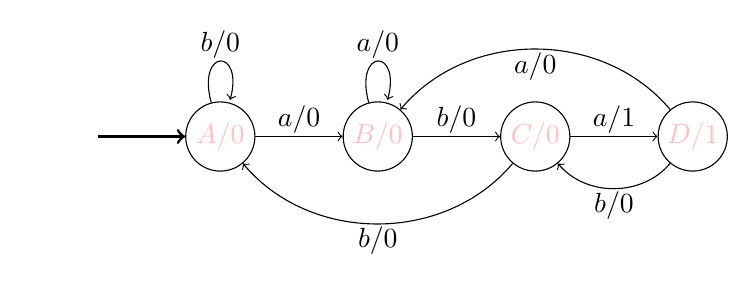
\begin{tikzpicture}[node distance = 2cm,auto,inner sep=1pt]
\node[state,draw=white,inner sep=0pt] (A) {$$};
\node[state,text=pink,draw=black] (B) [ right of = A]  {$A/0$};
\node[state,text=pink,draw=black] (C) [right of = B]  {$B/0$};
\node[state,text=pink,draw=black] (D) [right of = C]  {$C/0$};
\node[state,text=pink,draw=black] (E) [right of = D]  {$D/1$};

\path (A) edge [->,line width=1pt,node distance = 0.1cm] node {$$} (B);
\path (B) edge [->,loop above] node {$b/0$} (B);
\path (B) edge [->] node {$a/0$} (C);
\path (C) edge [->,loop above] node {$a/0$} (C);
\path (C) edge [->] node {$b/0$} (D);
\path (D) edge [->] node {$a/1$} (E);
\path (E) edge [->,bend left=50] node {$b/0$} (D);
\path (D) edge [->,bend left=50] node {$b/0$} (B);
\path (E) edge [->,bend right=50] node {$a/0$} (C);
\end{tikzpicture}
\end{center}
\begin{center}
\textbf{Fig. 3.35}
\end{center}

\vspace*{0.1cm}
\pause
\textbf{3.13.2.2 Mealy Machine to Moore Machine}

\vspace*{0.2cm}
For a given Mealy machine $M_C$, there is an equivalent Moore machine
$M_o$. These can be constructed in several steps.\\

\vspace*{0.2cm}
\end{frame}

\begin{frame}
\textbf{Step I:} In a Mealy machine, the output depends on the present state and
the present input. So, in the transactional diagram of a Mealy machine,
the transactional edges are labelled with input as well as output. For a
state, there two types of edges, namely, incoming edges and outgoing
edges. For incoming edges, it may happen that the output differs for two
incoming edges like the example shown in Fig. 3.36.\\

\pause
\begin{center}
\section{picture}
\includegraphics[width=5cm,height=3cm]{78-1.png}
\end{center}
\end{frame}

\begin{frame}
 \hspace*{0.2cm} In the transitional diagram for state S, the incoming edges are labelled
as $I_1/O_1$, $I_2/O_2$, and $I_2/O_1$, and the outgoing edges are labelled as $I_1/O_2$ and
$I_2/O_2$. For state S for incoming edges, we get two types of output $O_1$ and $O_2$. The state S is divided into n
number of parts, where $n = number$ of different outputs for the incoming edges to the state. The output
edges are repeated for all the divided states. The transitional diagram for this case is shown in Fig. 3.37.\\

\pause
\begin{center}
\section{picture}
\includegraphics[width=9cm,height=4cm]{78-2.png}
\end{center}
\end{frame}

\begin{frame}

\begin{flushright}
 \texttt{Finite State Machine} \hspace*{0.10cm}\textbf{$|$} \textbf{79}\hspace*{0.5cm}
\end{flushright}

\section*{Transitional Format}

\vspace*{1cm}

\textbf{Step II:} If a state has a loop like Fig. 3.38, that state also needs to be divided as shown in Fig. 3.39.

\begin{center}
\section{picture}
\includegraphics[width=9cm,height=3cm]{79.png}
\end{center}
[Here, for input $I_1$, the output is $O_1$ as well as $O_2$. So, the state S needs to be divided. S has a loop with
input $I_2$ and output $O_1$.]. The state S will be divided into two states $S_O1$ and $S_O2$.\\
\end{frame}

\begin{frame}
As the loop for input $I_2$
is labelled with output $O_1$, there will be a loop on state $S_O1$. But this loop is not possible on $S_O2$, because
it produces the output $O_2$. So, there will be a transition from $S_O2$ to $S_O1$ with input label $I_2$.\\

\vspace*{0.3cm}
\textbf{Step III:} Repeat the steps I and II. By this, the Moore machine equivalent to the Mealy machine is
constructed.\\
 \hspace*{0.3cm} The following examples (Examples 3.23 and 3.24) describe the process.\\
 
 \fcolorbox{red}{blue}{\textbf{Example 3.23}}\hspace*{0.1cm} \texttt{Convert the following Mealy machine
to an equivalent Moore machine as given in Fig. 3.40.}\\

\pause
\begin{center}
\section{picture}
\includegraphics[width=7cm,height=2.5cm]{79-1.png}
\end{center}
\end{frame}

\begin{frame}
\textbf{Solution:} For state $q_0$, there are two incoming states, $q_0$ to
$q_0$ with label $a/0$ and $q_2$ to $q_0$ with label $b/1$. Two incoming
edges are labelled with two different outputs $0$ and $1$. So,
the state $q_0$ needs to be divided into two states as $q_00$ and
$q_01$. A loop for input 'a' on $q_00$ is constructed. A transition
is made from $q_01$ to $q_00$ with input label 'a'. From both the
states, transitions are made to the state $q_1$ with label $b/1$.
The modified machine is given in Fig. 3.41.\\
\hspace*{0.3cm} For all the other states $q_1$ and $q_2$ the outputs for all the incoming edges are $1$ and $0$ respectively. So
there is no need to divide the states. The final Moore machine is as given in Fig. 3.42.
\pause
\begin{center}
\section{picture}
\includegraphics[width=9cm,height=3cm]{79-2.png}
\end{center}
\end{frame}

\begin{frame}
\section*{Transitional Format}
\begin{flushleft}
    \textbf{80}\hspace*{0.1cm} \textbf{$|$} \hspace*{0.1cm} \texttt{Introduction to Automata Theory, Formal Languages and Computation}
  \end{flushleft}

\vspace*{0.5cm}
 \fcolorbox{red}{blue}{\textbf{Example 3.23}}\hspace*{0.1cm} \texttt{Convert the following Mealy
machine as given in Fig. 3.43 to
an equivalent Moore machine.}\\

\pause
\begin{center}
\section{picture}
\includegraphics[width=8cm,height=3cm]{80-1.png}
\end{center}
\end{frame}

\begin{frame}
Solution: The machine contains four states. Let us
start from the state $q_1$. The incoming edges to this
state are from $q_2$ to $q_1$ with label $0/1$ and from $q_3$ to $q_1$
with label $1/1$. There is no difference in the outputs
of the incoming edges to this state and, therefore,
in the constructing Moore machine, the output for
this state is $1$. The modified machine is as shown in
Fig. 3.44.\\

\pause
\begin{center}
\section{picture}
\includegraphics[width=8cm,height=3cm]{80-2.png}
\end{center}
\end{frame}

\begin{frame}
\hspace*{0.3cm} Consider the state $q_2$. This state contains two
incoming edges: from $q_1$ to $q_2$ with label $1/0$ and $q_3$
to $q_2$ with label $0/1$. We get two different outputs
for the two incoming edges ($q_1$ to $q_2$ output $0$, $q_3$
to $q_2$ output $1$). So, the state $q_2$ is divided into two,
namely, $q_20$ and $q_21$. The outgoing edges are duplicated
for both the states generated from $q_2$ as shown
in Fig. 3.45.\\

\pause
\begin{center}
\section{picture}
\includegraphics[width=8cm,height=4cm]{80-3.png}
\end{center}
\end{frame}

\begin{frame}
Consider the state $q_3$. The incoming edges to this state are from $q_1$ to $q_3$ with label $0/0$ and from $q_4$ to $q_3$
with label $1/0$. There is no difference in the outputs of the incoming edges to this state and, therefore,
in the constructing Moore machine, the output for this state is $0$. The modified machine is given in
Fig. 3.46.\\
\hspace*{0.3cm} Consider the state $q_4$. This state contains three incoming edges, from $q_20$ to $q_4$ with label $1/0$, from $q_21$ to
$q_4$ with label $1/0$, and from and $q_4$ to $q_4$ with label $0/1$. We get two different outputs for the three incoming
edges ($q_20$ to $q_4$ output $0$, $q_21$ to $q_4$ output $0$, and $q_4$ to $q_4$ output $1$). So, the state $q_4$ will be divided into two,
namely, $q_40$ and $q_41$.\\
\hspace*{0.3cm} The modified Moore machine is given in Fig. 3.47.
\end{frame}
\end{document} 